\section{Einführung}
Ich arbeite als GIS-Spezialist bei der swisstopo\footnote{\href{https://www.swisstopo.ch}{www.swisstopo.ch}}, dem Bundesamt für Landestopografie in Wabern. Wir machen Karten. Mein Team macht Internetkarten - wie Google Maps\footnote{\href{https://maps.google.com}{maps.google.com}}, jedoch von der Schweiz für die Schweiz; und für alle anderen auch. Unsere Internetkarte, der Viewer, erfreut sich relativ grosser Beliebtheit
und beinhaltet ca. 800 Themen wie Wanderwege, Solarkataster oder Luftfahrthindernisse. Lieber Leser\footnote{Im vorliegenden Dokument wird durchwegs der männliche Singular (Leser, Benutzer) als Ansprache verwendet. Diese Ansprache bezieht sich auf beide Geschlechter sowie gegebenenfalls mehrere Personen. Sie dient lediglich der leichteren Lesbarkeit der Semesterarbeit}, falls dir \href{https://map.geo.admin.ch}{map.geo.admin.ch} noch kein Begriff sein sollte, kann ich dir wärmstens empfehlen, dir etwas Zeit zu nehmen, um darin zu schmökern. Es gibt viel zu entdecken und es gratis - ein Service Public.

\begin{figure}[H]
	\centering
	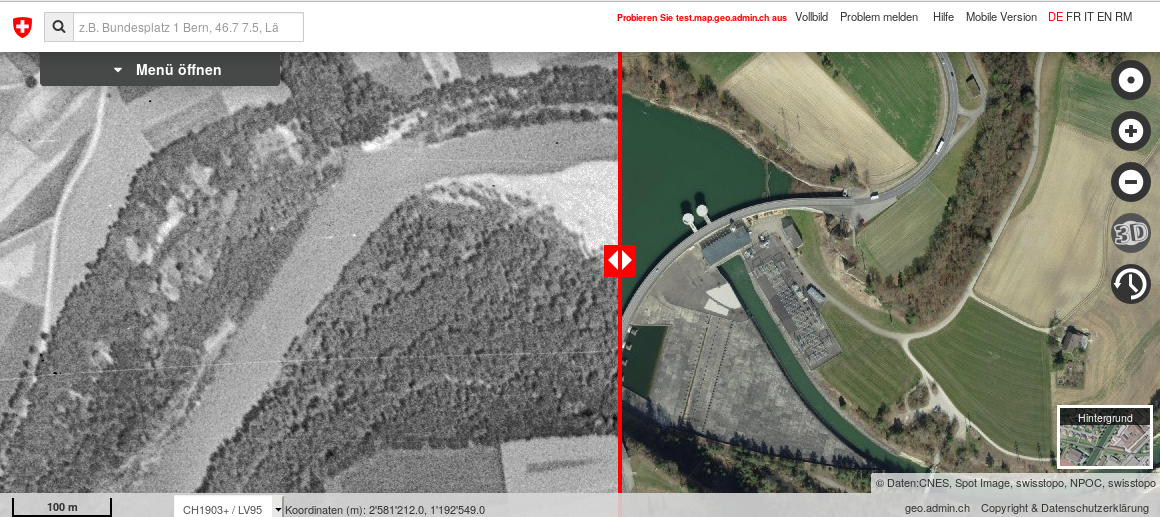
\includegraphics[width=.95\textwidth]{hist_map_geo_admin}
	\caption{Internetkarte des Bundes \emph{\href{https://s.geo.admin.ch/8a82499889}{map.geo.admin.ch}}. Hier ein Ausschnitt der Saane bei Kleinbösingen, das Luftaufnahmen von 1946 zu heute vergleicht.}
	\label{fig:map.geo.admin.ch}
\end{figure}


\subsection{GIS}
Wie erwähnt, arbeite ich als \emph{GIS-Spezialist}. Wobei mir der Titel \emph{Geo-Informatiker} besser gefällt: weil er \emph{Geografie} und \emph{Informatik} beinhaltet. \emph{Geografie} kommt aus dem Griechischen und bedeutet Erdbeschreibung. \emph{Informatik} ist die Wissenschaft von der systematischen Darstellung, Speicherung, Verarbeitung und Übertragung von Informationen.

GIS ist ein Akronym für Geographical Information Systems. GIS bedeutet im engsten Sinn eine Ansammlung von Computerprogrammen, die zur Bearbeitung von Karten und Geodaten verwendet werden. Geodaten sind nichts weiter als Daten mit einem räumlichen Bezug\footnote{mit Koordinaten, typisch Nord und Ost}. In einem weiteren Sinn deckt der Begriff GIS ein ganzes Fachgebiet ab, das sich mit Karten und Geodaten auskennt. Es ist also nicht nur ein Werkzeug, sondern ein Fachgebiet, das Kenntnisse über Datensammlung, Speicherung, Analyse und Darstellung innerhalb von vielen verschiedenen Themen mit einem räumlichen Bezug abdeckt. 

Es ist zwar weit von der klassischen Geografie zu Zeiten Humbolds entfernt, aber es liegt auf der Hand, dass auch Cloud Computing zu GIS gehört.



Typische Geodaten sind digitale Karten, Inventare und Register von Parzellen, Umweltfaktoren, Grenzen, Entwicklung, Planung etc., die einen räumlichen Bezug haben und dadurch in einem geografischen Zusammenhang analysiert und dargestellt werden können.

Unser
Team (IGEB-B) publiziert diese Daten; deren Nachführungszyklus wie auch der Aufwand zur
Aufbereitung fürs Web unterschiedlich sind. Einige Daten werden manuell aufbereitet, andere
stündlich automatisch nachgeführt.

